% eviction_ratio.tex: evictions of conflict-free placements of rising access imbalance, relative to the balanced
% placement, in sixteen cached banks (generated by make_eviction_ratio.py). Full width.
% Needs: \usepackage{pgfplots} \pgfplotsset{compat=1.17} \usepgfplotslibrary{fillbetween}
\begin{figure*}[!t]
\centering
{%
\definecolor{iA}{HTML}{F4A582}\definecolor{iB}{HTML}{D6604D}\definecolor{iC}{HTML}{B2182B}\definecolor{iD}{HTML}{67001F}%
\pgfplotsset{eA/.style={iA, line width=0.9pt, densely dashed, mark=square*, mark size=1.2pt, mark options={solid}}, eAc/.style={fill=iA},
  eB/.style={iB, line width=0.9pt, dotted, mark=triangle*, mark size=1.4pt, mark options={solid}}, eBc/.style={fill=iB},
  eC/.style={iC, line width=0.9pt, dash dot, mark=diamond*, mark size=1.4pt, mark options={solid}}, eCc/.style={fill=iC},
  eD/.style={iD, line width=0.9pt, mark=pentagon*, mark size=1.4pt}, eDc/.style={fill=iD}}%
\begin{tikzpicture}
\begin{axis}[width=0.345\textwidth, height=0.26\textwidth, axis lines=box, axis line style={black, line width=0.5pt}, tick align=inside, tick style={black!70},
  ymode=log, log basis y=2, ymin=0.8, ymax=64, ytick={1,2,4,8,16,32}, yticklabels={1,2,4,8,16,32},
  grid=both, major grid style={black!40, dotted, line width=0.5pt}, minor grid style={black!15, dotted, line width=0.4pt},
  tick label style={font=\scriptsize}, label style={font=\footnotesize}, title style={font=\footnotesize},
  ylabel style={yshift=-4pt},
  legend style={font=\tiny, draw=black!60, fill=white, fill opacity=0.9, text opacity=1, legend cell align=left}, xmode=log, log basis x=2, xmin=200, xmax=80000,
  xtick={256,1024,4096,16384,65536}, xticklabels={$2^{8}$,$2^{10}$,$2^{12}$,$2^{14}$,$2^{16}$},
  xlabel={Cache Lines per Bank}, ylabel={Evictions vs.\ Balanced}, title={(a) RouteViews trie},
  legend style={at={(0.03,0.97)}, anchor=north west}]
  \draw[black!60, densely dashed, line width=0.6pt] (axis cs:200,1) -- (axis cs:80000,1);
  \addplot[draw=none, name path=trie8lo, forget plot] table[x=x, y=lo]{
x med lo hi
256 0.9960 0.9938 0.9980
512 0.9922 0.9890 0.9945
1024 0.9907 0.9873 0.9934
2048 0.9920 0.9867 0.9965
4096 0.9976 0.9905 1.0069
8192 1.0178 1.0077 1.1331
16384 1.1030 1.0638 1.4331
32768 1.4854 1.3063 1.8868
65536 2.1489 1.8989 2.4685
};
  \addplot[draw=none, name path=trie8hi, forget plot] table[x=x, y=hi]{
x med lo hi
256 0.9960 0.9938 0.9980
512 0.9922 0.9890 0.9945
1024 0.9907 0.9873 0.9934
2048 0.9920 0.9867 0.9965
4096 0.9976 0.9905 1.0069
8192 1.0178 1.0077 1.1331
16384 1.1030 1.0638 1.4331
32768 1.4854 1.3063 1.8868
65536 2.1489 1.8989 2.4685
};
  \addplot[eAc, fill opacity=0.16, draw=none, forget plot] fill between[of=trie8lo and trie8hi];
  \addplot[eA] table[x=x, y=med]{
x med lo hi
256 0.9960 0.9938 0.9980
512 0.9922 0.9890 0.9945
1024 0.9907 0.9873 0.9934
2048 0.9920 0.9867 0.9965
4096 0.9976 0.9905 1.0069
8192 1.0178 1.0077 1.1331
16384 1.1030 1.0638 1.4331
32768 1.4854 1.3063 1.8868
65536 2.1489 1.8989 2.4685
};
  \addlegendentry{54\%}
  \addplot[draw=none, name path=trie4lo, forget plot] table[x=x, y=lo]{
x med lo hi
256 0.9898 0.9868 0.9927
512 0.9803 0.9770 0.9838
1024 0.9758 0.9714 0.9794
2048 0.9868 0.9815 0.9917
4096 1.0076 1.0011 1.0161
8192 1.0560 1.0432 1.2590
16384 1.1894 1.1389 1.7859
32768 1.8611 1.5193 2.6375
65536 3.2973 2.7499 3.9877
};
  \addplot[draw=none, name path=trie4hi, forget plot] table[x=x, y=hi]{
x med lo hi
256 0.9898 0.9868 0.9927
512 0.9803 0.9770 0.9838
1024 0.9758 0.9714 0.9794
2048 0.9868 0.9815 0.9917
4096 1.0076 1.0011 1.0161
8192 1.0560 1.0432 1.2590
16384 1.1894 1.1389 1.7859
32768 1.8611 1.5193 2.6375
65536 3.2973 2.7499 3.9877
};
  \addplot[eBc, fill opacity=0.16, draw=none, forget plot] fill between[of=trie4lo and trie4hi];
  \addplot[eB] table[x=x, y=med]{
x med lo hi
256 0.9898 0.9868 0.9927
512 0.9803 0.9770 0.9838
1024 0.9758 0.9714 0.9794
2048 0.9868 0.9815 0.9917
4096 1.0076 1.0011 1.0161
8192 1.0560 1.0432 1.2590
16384 1.1894 1.1389 1.7859
32768 1.8611 1.5193 2.6375
65536 3.2973 2.7499 3.9877
};
  \addlegendentry{77\%}
  \addplot[draw=none, name path=trie2lo, forget plot] table[x=x, y=lo]{
x med lo hi
256 0.9842 0.9818 0.9865
512 0.9713 0.9684 0.9744
1024 0.9764 0.9734 0.9805
2048 0.9952 0.9894 1.0001
4096 1.0239 1.0165 1.0336
8192 1.0806 1.0660 1.3315
16384 1.2535 1.1820 1.9984
32768 2.0871 1.6370 3.0728
65536 3.9488 3.3273 4.9395
};
  \addplot[draw=none, name path=trie2hi, forget plot] table[x=x, y=hi]{
x med lo hi
256 0.9842 0.9818 0.9865
512 0.9713 0.9684 0.9744
1024 0.9764 0.9734 0.9805
2048 0.9952 0.9894 1.0001
4096 1.0239 1.0165 1.0336
8192 1.0806 1.0660 1.3315
16384 1.2535 1.1820 1.9984
32768 2.0871 1.6370 3.0728
65536 3.9488 3.3273 4.9395
};
  \addplot[eCc, fill opacity=0.16, draw=none, forget plot] fill between[of=trie2lo and trie2hi];
  \addplot[eC] table[x=x, y=med]{
x med lo hi
256 0.9842 0.9818 0.9865
512 0.9713 0.9684 0.9744
1024 0.9764 0.9734 0.9805
2048 0.9952 0.9894 1.0001
4096 1.0239 1.0165 1.0336
8192 1.0806 1.0660 1.3315
16384 1.2535 1.1820 1.9984
32768 2.0871 1.6370 3.0728
65536 3.9488 3.3273 4.9395
};
  \addlegendentry{88\%}
  \addplot[draw=none, name path=trie1lo, forget plot] table[x=x, y=lo]{
x med lo hi
256 0.9829 0.9807 0.9855
512 0.9742 0.9712 0.9771
1024 0.9857 0.9813 0.9896
2048 1.0119 1.0063 1.0178
4096 1.0285 1.0216 1.0390
8192 1.0878 1.0759 1.3604
16384 1.2900 1.1995 2.0592
32768 2.3166 1.7412 3.4838
65536 5.0131 3.9274 7.1700
};
  \addplot[draw=none, name path=trie1hi, forget plot] table[x=x, y=hi]{
x med lo hi
256 0.9829 0.9807 0.9855
512 0.9742 0.9712 0.9771
1024 0.9857 0.9813 0.9896
2048 1.0119 1.0063 1.0178
4096 1.0285 1.0216 1.0390
8192 1.0878 1.0759 1.3604
16384 1.2900 1.1995 2.0592
32768 2.3166 1.7412 3.4838
65536 5.0131 3.9274 7.1700
};
  \addplot[eDc, fill opacity=0.16, draw=none, forget plot] fill between[of=trie1lo and trie1hi];
  \addplot[eD] table[x=x, y=med]{
x med lo hi
256 0.9829 0.9807 0.9855
512 0.9742 0.9712 0.9771
1024 0.9857 0.9813 0.9896
2048 1.0119 1.0063 1.0178
4096 1.0285 1.0216 1.0390
8192 1.0878 1.0759 1.3604
16384 1.2900 1.1995 2.0592
32768 2.3166 1.7412 3.4838
65536 5.0131 3.9274 7.1700
};
  \addlegendentry{92\%}
\end{axis}
\end{tikzpicture}\hfill
\begin{tikzpicture}
\begin{axis}[width=0.345\textwidth, height=0.26\textwidth, axis lines=box, axis line style={black, line width=0.5pt}, tick align=inside, tick style={black!70},
  ymode=log, log basis y=2, ymin=0.8, ymax=64, ytick={1,2,4,8,16,32}, yticklabels={1,2,4,8,16,32},
  grid=both, major grid style={black!40, dotted, line width=0.5pt}, minor grid style={black!15, dotted, line width=0.4pt},
  tick label style={font=\scriptsize}, label style={font=\footnotesize}, title style={font=\footnotesize},
  ylabel style={yshift=-4pt},
  legend style={font=\tiny, draw=black!60, fill=white, fill opacity=0.9, text opacity=1, legend cell align=left}, xmode=log, log basis x=2, xmin=200, xmax=80000,
  xtick={256,1024,4096,16384,65536}, xticklabels={$2^{8}$,$2^{10}$,$2^{12}$,$2^{14}$,$2^{16}$},
  xlabel={Cache Lines per Bank}, ylabel={Evictions vs.\ Balanced}, title={(b) Prioritised replay},
  legend style={at={(0.03,0.97)}, anchor=north west}]
  \draw[black!60, densely dashed, line width=0.6pt] (axis cs:200,1) -- (axis cs:80000,1);
  \addplot[draw=none, name path=rep8lo, forget plot] table[x=x, y=lo]{
x med lo hi
256 0.9867 0.9842 0.9882
512 0.9895 0.9880 0.9907
1024 0.9909 0.9888 0.9928
2048 1.0147 1.0117 1.0192
4096 1.0126 1.0096 1.0208
8192 1.0726 1.0672 1.0830
16384 1.1641 1.1525 1.5245
32768 1.6382 1.5449 3.4837
65536 3.2349 2.8787 4.8859
};
  \addplot[draw=none, name path=rep8hi, forget plot] table[x=x, y=hi]{
x med lo hi
256 0.9867 0.9842 0.9882
512 0.9895 0.9880 0.9907
1024 0.9909 0.9888 0.9928
2048 1.0147 1.0117 1.0192
4096 1.0126 1.0096 1.0208
8192 1.0726 1.0672 1.0830
16384 1.1641 1.1525 1.5245
32768 1.6382 1.5449 3.4837
65536 3.2349 2.8787 4.8859
};
  \addplot[eAc, fill opacity=0.16, draw=none, forget plot] fill between[of=rep8lo and rep8hi];
  \addplot[eA] table[x=x, y=med]{
x med lo hi
256 0.9867 0.9842 0.9882
512 0.9895 0.9880 0.9907
1024 0.9909 0.9888 0.9928
2048 1.0147 1.0117 1.0192
4096 1.0126 1.0096 1.0208
8192 1.0726 1.0672 1.0830
16384 1.1641 1.1525 1.5245
32768 1.6382 1.5449 3.4837
65536 3.2349 2.8787 4.8859
};
  \addlegendentry{78\%}
  \addplot[draw=none, name path=rep4lo, forget plot] table[x=x, y=lo]{
x med lo hi
256 0.9923 0.9908 0.9942
512 1.0235 1.0215 1.0258
1024 1.0582 1.0564 1.0618
2048 1.0252 1.0225 1.0304
4096 1.0545 1.0507 1.0637
8192 1.1557 1.1503 1.1738
16384 1.3095 1.2979 1.8724
32768 2.0430 1.9032 6.0698
65536 6.0409 4.7989 20.2026
};
  \addplot[draw=none, name path=rep4hi, forget plot] table[x=x, y=hi]{
x med lo hi
256 0.9923 0.9908 0.9942
512 1.0235 1.0215 1.0258
1024 1.0582 1.0564 1.0618
2048 1.0252 1.0225 1.0304
4096 1.0545 1.0507 1.0637
8192 1.1557 1.1503 1.1738
16384 1.3095 1.2979 1.8724
32768 2.0430 1.9032 6.0698
65536 6.0409 4.7989 20.2026
};
  \addplot[eBc, fill opacity=0.16, draw=none, forget plot] fill between[of=rep4lo and rep4hi];
  \addplot[eB] table[x=x, y=med]{
x med lo hi
256 0.9923 0.9908 0.9942
512 1.0235 1.0215 1.0258
1024 1.0582 1.0564 1.0618
2048 1.0252 1.0225 1.0304
4096 1.0545 1.0507 1.0637
8192 1.1557 1.1503 1.1738
16384 1.3095 1.2979 1.8724
32768 2.0430 1.9032 6.0698
65536 6.0409 4.7989 20.2026
};
  \addlegendentry{126\%}
  \addplot[draw=none, name path=rep2lo, forget plot] table[x=x, y=lo]{
x med lo hi
256 1.2456 1.2415 1.2510
512 1.3503 1.3456 1.3573
1024 1.0524 1.0503 1.0552
2048 1.0415 1.0385 1.0456
4096 1.0736 1.0707 1.0800
8192 1.1761 1.1695 1.1949
16384 1.3521 1.3380 1.9967
32768 2.1799 2.0396 8.2310
65536 7.2099 5.6688 31.8221
};
  \addplot[draw=none, name path=rep2hi, forget plot] table[x=x, y=hi]{
x med lo hi
256 1.2456 1.2415 1.2510
512 1.3503 1.3456 1.3573
1024 1.0524 1.0503 1.0552
2048 1.0415 1.0385 1.0456
4096 1.0736 1.0707 1.0800
8192 1.1761 1.1695 1.1949
16384 1.3521 1.3380 1.9967
32768 2.1799 2.0396 8.2310
65536 7.2099 5.6688 31.8221
};
  \addplot[eCc, fill opacity=0.16, draw=none, forget plot] fill between[of=rep2lo and rep2hi];
  \addplot[eC] table[x=x, y=med]{
x med lo hi
256 1.2456 1.2415 1.2510
512 1.3503 1.3456 1.3573
1024 1.0524 1.0503 1.0552
2048 1.0415 1.0385 1.0456
4096 1.0736 1.0707 1.0800
8192 1.1761 1.1695 1.1949
16384 1.3521 1.3380 1.9967
32768 2.1799 2.0396 8.2310
65536 7.2099 5.6688 31.8221
};
  \addlegendentry{161\%}
  \addplot[draw=none, name path=rep1lo, forget plot] table[x=x, y=lo]{
x med lo hi
256 1.4452 1.4403 1.4534
512 1.3286 1.3226 1.3346
1024 1.0014 0.9997 1.0030
2048 1.0196 1.0173 1.0219
4096 1.0686 1.0657 1.0715
8192 1.1726 1.1667 1.1926
16384 1.3462 1.3352 2.0059
32768 2.2499 2.0905 9.2450
65536 8.1628 6.3423 46.5052
};
  \addplot[draw=none, name path=rep1hi, forget plot] table[x=x, y=hi]{
x med lo hi
256 1.4452 1.4403 1.4534
512 1.3286 1.3226 1.3346
1024 1.0014 0.9997 1.0030
2048 1.0196 1.0173 1.0219
4096 1.0686 1.0657 1.0715
8192 1.1726 1.1667 1.1926
16384 1.3462 1.3352 2.0059
32768 2.2499 2.0905 9.2450
65536 8.1628 6.3423 46.5052
};
  \addplot[eDc, fill opacity=0.16, draw=none, forget plot] fill between[of=rep1lo and rep1hi];
  \addplot[eD] table[x=x, y=med]{
x med lo hi
256 1.4452 1.4403 1.4534
512 1.3286 1.3226 1.3346
1024 1.0014 0.9997 1.0030
2048 1.0196 1.0173 1.0219
4096 1.0686 1.0657 1.0715
8192 1.1726 1.1667 1.1926
16384 1.3462 1.3352 2.0059
32768 2.2499 2.0905 9.2450
65536 8.1628 6.3423 46.5052
};
  \addlegendentry{187\%}
\end{axis}
\end{tikzpicture}\hfill
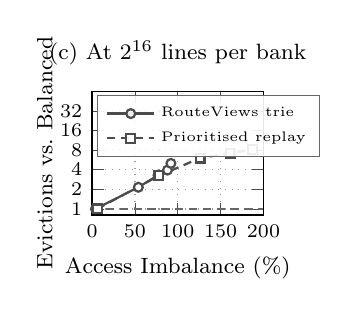
\begin{tikzpicture}
\begin{axis}[width=0.31\textwidth, height=0.26\textwidth, axis lines=box, axis line style={black, line width=0.5pt}, tick align=inside, tick style={black!70},
  ymode=log, log basis y=2, ymin=0.8, ymax=64, ytick={1,2,4,8,16,32}, yticklabels={1,2,4,8,16,32},
  grid=both, major grid style={black!40, dotted, line width=0.5pt}, minor grid style={black!15, dotted, line width=0.4pt},
  tick label style={font=\scriptsize}, label style={font=\footnotesize}, title style={font=\footnotesize},
  ylabel style={yshift=-4pt},
  legend style={font=\tiny, draw=black!60, fill=white, fill opacity=0.9, text opacity=1, legend cell align=left}, xmin=0, xmax=200, xtick={0,50,100,150,200},
  xlabel={Access Imbalance (\%)}, ylabel={Evictions vs.\ Balanced}, title={(c) At $2^{16}$ lines per bank},
  legend style={at={(0.03,0.97)}, anchor=north west}]
  \draw[black!60, densely dashed, line width=0.6pt] (axis cs:0,1) -- (axis cs:200,1);
  \addplot[black!70, line width=0.8pt, mark=*, mark size=1.6pt, mark options={solid, fill=white}] coordinates {(4,1.0000) (54,2.1489) (77,3.2973) (88,3.9488) (92,5.0131)};
  \addlegendentry{RouteViews trie}
  \addplot[black!70, line width=0.8pt, densely dashed, mark=square*, mark size=1.6pt, mark options={solid, fill=white}] coordinates {(6,1.0000) (78,3.2349) (126,6.0409) (161,7.2099) (187,8.1628)};
  \addlegendentry{Prioritised replay}
\end{axis}
\end{tikzpicture}%
}
\caption{Evictions of conflict-free placements of rising access imbalance, relative to the balanced placement, in sixteen cached banks: (a, b)~against cache size, (c)~against imbalance at the largest cache.}
\label{fig:evictions}
\end{figure*}
